\section{Muhammad Reza Syachrani - 1174084}
\subsection{Teori}
\begin{enumerate}

	\item Jelaskan kenapa file teks harus di lakukan tokenizer. dilengkapi dengan ilustrasi atau gambar
	\hfill\\
untuk mempermudah mesin dalam mengolah file teks yang dimana bentuk teks tersebut di konversi menjadi urutan integer kata atau vector binary. ilustrasi tokenizer sebagai berikut, saya memiliki teks yaitu "saya makan nasi goreng" dan setelah dilakukan tokenizer berubah menjadi {'saya': 1, 'makan': 2, 'nasi': 3, 'goreng': 4}

\item Jelaskan konsep dasar K Fold Cross Validation pada dataset komentar Youtube.
	\hfill\\
	pada codingan tersebut terdapat variabel kfold yang berisi fungsi StratifiedKFold yang memiliki parameter n\_splits=5 yang berarti melakukan pengulangan terhadap data masing-masing lima kali dengan atribut class sebagai acuan pengolahan datanya kemudian akan di hasilkan akurasi dari pengulangan data tersebut sebesar sekian persen tergantung datanya. 

\begin{figure}[H]
    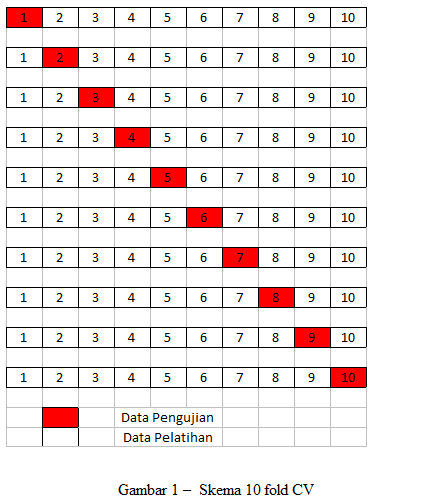
\includegraphics[width=12cm]{figures/1174084/7/teori2.png}
    \centering
    \caption{Teori 2}
\end{figure}

\item Jelaskan apa maksudnya kode program for train, test in splits.dilengkapi dengan ilustrasi atau gambar.
	\hfill\\
	kode program for train fungsinya untuk melakukan training terhadap data yang telah di deklarasikan sebelumnya. sedangkan kode program test in split fungsinya untuk membatasi jumlah data yang akan digunakan.

\begin{figure}[H]
    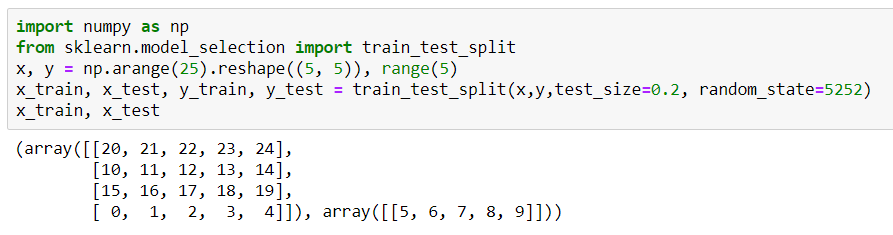
\includegraphics[width=12cm]{figures/1174084/7/teori3.png}
    \centering
    \caption{Teori 3}
\end{figure}

\item Jelaskan apa maksudnya kode program train\_content = d[’CONTENT’].iloc[train idx] dan test\_content = d[’CONTENT’].iloc[test idx]. dilengkapi dengan ilustrasi atau gambar.
\hfill\\
	kode program train content tersebut adalah membaca isian kolom pada field yang bernama CONTENT sebagai data training sedangkan kode program test content membaca isi kolom pada field yang bernama CONTENT sebagai data testing.
	
\begin{figure}[H]
    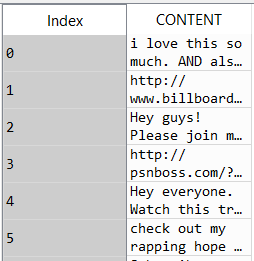
\includegraphics[width=8cm]{figures/1174084/7/teori4.png}
    \centering
    \caption{Teori 4}
\end{figure}

\item Jelaskan apa maksud dari fungsi tokenizer = Tokenizer(num\_words=2000) dan tokenizer.fit\_on\_texts(train\_content), dilengkapi dengan ilustrasi atau gambar.
	\hfill\\
fungsi tokenizer = Tokennizer(num\_words=2000) untuk membaca kalimat menjadi token/indeks sebanyak 2000 kata dan fungsi fit\_on\_texts(train\_konten) untuk membuat membaca data token/indeks teks yang telah di masukan kedalam data train\_konten.

\begin{figure}[H]
    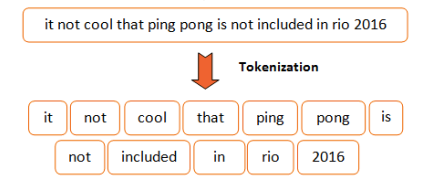
\includegraphics[width=8cm]{figures/1174084/7/teori5.png}
    \centering
    \caption{Teori 5}
\end{figure}

\item Jelaskan apa maksud dari fungsi d\_train\_inputs = tokenizer.texts\_to\_matrix(train\_content, mode=’tfidf’) dan d\_test\_inputs = tokenizer.texts\_to\_matrix(test\_content, mode=’tfidf’), dilengkapi dengan ilustrasi kode dan atau gambar
	\hfill\\
	variabel d\_train\_inputs melakukan tokenizer dari bentuk teks menjadi bentuk matrix yang berurutan dari data train\_content dengan mode tf idf begitu juga dengan d\_test\_inputs untuk data test.
	
\begin{figure}[H]
    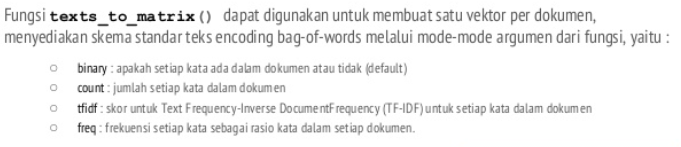
\includegraphics[width=8cm]{figures/1174084/7/teori6.png}
    \centering
    \caption{Teori 6}
\end{figure}

\item Jelaskan apa maksud dari fungsi d\_train\_inputs = d\_train\_inputs/np.amax(np.absolute(d\_train dan d\_test\_inputs = d\_test\_inputs/np.amax(np.absolute(d\_test\_inputs)), dilengkapi dengan ilustrasi atau gambar.
	\hfill\\
	fungsi tersebut digunakan untuk membagi matrix tfidf untuk menentukan maksimum array yang kemudian hasilnya tersebut dimasukan ke dalam variabel d\_train\_input dan d\_test\_input dengan metode absolute sehingga tanpa adanya bilangan negatif dan nol.
		
\begin{figure}[H]
    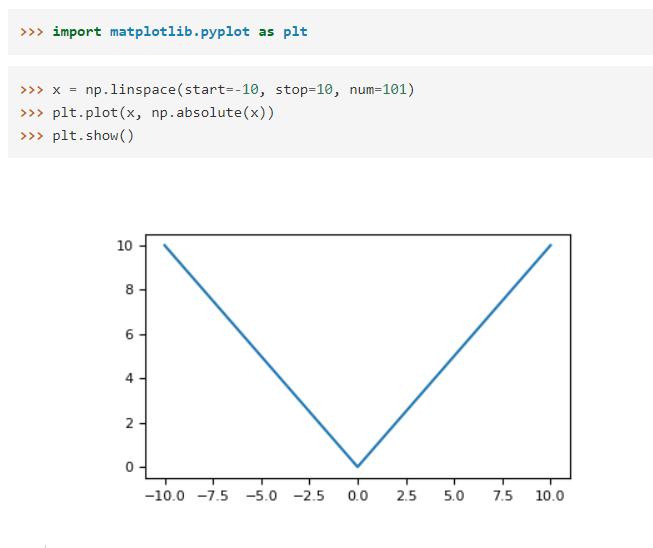
\includegraphics[width=8cm]{figures/1174084/7/teori7.png}
    \centering
    \caption{Teori 7}
\end{figure}

\item Jelaskan apa maksud fungsi dari d\_train\_outputs = np\_utils.to\_categorical(d[’CLASS’].iloc[train\_idx] dan d\_test\_outputs = np\_utils.to\_categorical(d[’CLASS’].iloc[test\_idx]) dalam kode program, dilengkapi dengan ilustrasi atau gambar.
	\hfill\\
	fungsi untuk melakukan one-hot encoding merubah nilai vektor dengan bentuk integer yang ada pada atribut class menjadi bentuk matrix biner untuk atribut CLASS sehingga hanya ada dua pilihan yaitu 0 atau 1.
	
\begin{figure}[H]
    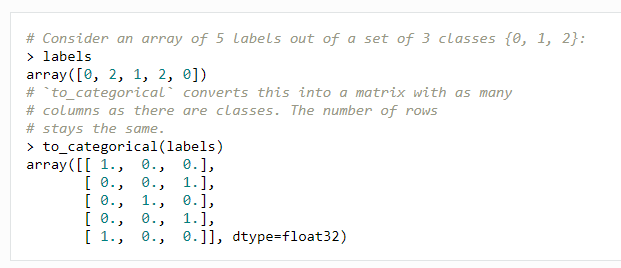
\includegraphics[width=8cm]{figures/1174084/7/teori8.png}
    \centering
    \caption{Teori 8}
\end{figure}


\item Jelaskan apa maksud dari fungsi di listing 7.2. Gambarkan ilustrasi Neural Network nya dari model kode tersebut.
	\hfill\\
	fungsi kode tersebut untuk melakukan permodelan sequential yang digunakan untuk mencari data dengan menerima parameter atau argumen kunci. kemudian di tambhakan metod add dengan danse sebanyak 512 neuron inputan dengan input shape 2000 vektor yang sudah dinormalisasi. kemudian di tambahkan lagi fungsi aktivasi dengan fungsi "relu". dan dilakukan overfitting atau pemotongan bobot sebesar 0.5 atau 50 persen.  Lalu pada layer output terdapat 2 neuron output. Kemudian outputan tersebut diaktivasi menggunakan fungsi softmax.
	
\begin{figure}[H]
    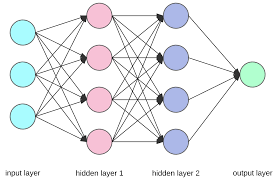
\includegraphics[width=8cm]{figures/1174084/7/teori9.png}
    \centering
    \caption{Teori 9}
\end{figure}


\item Jelaskan apa maksud dari fungsi di listing 7.3 dengan parameter tersebut.
	\hfill\\
	fungsi kode yang melakukan compile pada model dengan menggunakan beberapa parameter seperti loss yang akan mengembalikan fungsi nilai loss yang diambil, sedangkan fungsi adamax digunakan untuk mengetahui nilai lossnya, dan matrics = akurasi merupakan akurasi dari nilai matriknya.	
	

\item Jelaskan apa itu Deep Learning
	\hfill\\
	Merupakan metode pada machine learning yang menggunakan artificial neural networks. algoritma permodelan abstraksi tingkat tinggi pada data menggunakan sekumpulan fungsi transformasi non-linear yang ditata berlapis-lapis dan mendalam.
	

\item Jelaskan apa itu Deep Neural Network, dan apa bedanya dengan Deep Learning
	\hfill\\
	Deep Neural Network merupakan algoritma jaringan syaraf yang akan melakukan pembobotan terhadap data yang sudah ada sebagai acuan untuk data inputan selanjutnya. kemudian terdiri atas beberapa lapisan/layar atau hiden layer. perbedaan antara deep learning dan Deep Neural Network yaitu Deep Neural Network merupakan algoritma sedangkan deep learning yang menggunakan Deep Neural Network tersebut.


\item Jelaskan dengan ilustrasi gambar buatan sendiri(langkah per langkah) bagaimana perhitungan algoritma konvolusi dengan ukuran stride (NPM mod3+1) x (NPM mod3+1) yang terdapat max pooling
	\hfill\\
	Karena NPM saya 1164084 dan hasil dari (NPM mod 3)+1 = 2, maka saya menggunaan stride 2 dengan ketentuan max pooling 2x2.
	
\begin{figure}[H]
    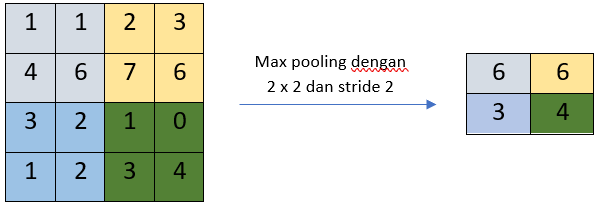
\includegraphics[width=8cm]{figures/1174084/7/teori10.png}
    \centering
    \caption{Teori 13}
\end{figure}
\end{enumerate}




\subsection{Praktek}
\begin{enumerate}

\item Jelaskan kode program pada blok In[1]
\lstinputlisting[firstline=8, lastline=15]{src/1174084/7/1174084.py}
\begin{figure}[H]
	\centering
	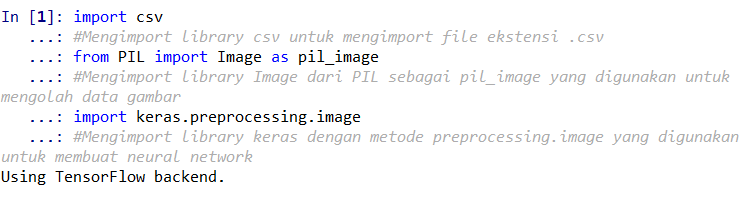
\includegraphics[width=10cm]{figures/1174084/7/1.png}
	\caption{Hasil Praktek 1}
\end{figure}

\item Jelaskan kode program pada blok In[2].
\lstinputlisting[firstline=16, lastline=44]{src/1174084/7/1174084.py}
\begin{figure}[H]
	\centering
	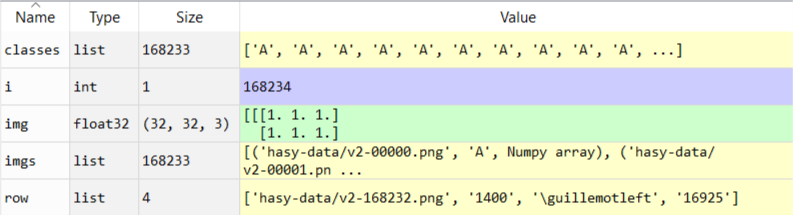
\includegraphics[width=10cm]{figures/1174084/7/2.png}
	\caption{Hasil Praktek 2}
\end{figure}

\item Jelaskan kode program pada blok In[3]
\lstinputlisting[firstline=45, lastline=57]{src/1174084/7/1174084.py}
\begin{figure}[H]
	\centering
	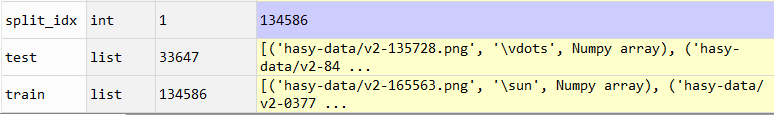
\includegraphics[width=10cm]{figures/1174084/7/3.png}
	\caption{Hasil Praktek 3}
\end{figure}

\item Jelaskan kode program pada blok  In[4]
\lstinputlisting[firstline=58, lastline=74]{src/1174084/7/1174084.py}
\begin{figure}[H]
	\centering
	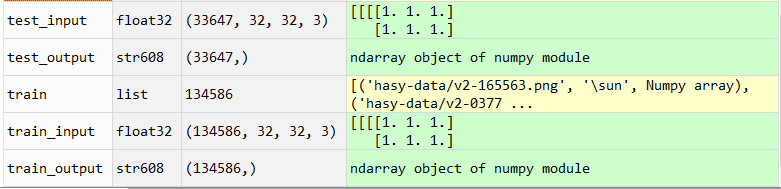
\includegraphics[width=10cm]{figures/1174084/7/4.png}
	\caption{Hasil Praktek 4}
\end{figure}

\item Jelaskan kode program pada blok  In[5]
\lstinputlisting[firstline=75, lastline=80]{src/1174084/7/1174084.py}
\begin{figure}[H]
	\centering
	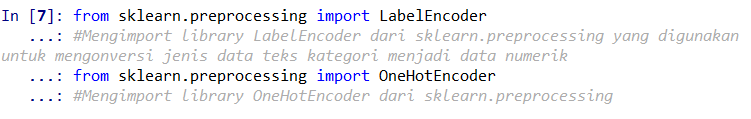
\includegraphics[width=10cm]{figures/1174084/7/5.png}
	\caption{Hasil Praktek 5}
\end{figure}

\item Jelaskan kode program pada blok  In[6]
\lstinputlisting[firstline=81, lastline=88]{src/1174084/7/1174084.py}		
\begin{figure}[H]
    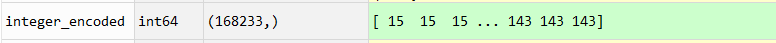
\includegraphics[width=8cm]{figures/1174084/7/6.png}
    \centering
    \caption{Hasil Praktek 6}
\end{figure}


\item Jelaskan kode program pada blok In[7]
\lstinputlisting[firstline=89, lastline=96]{src/1174084/7/1174084.py}
\begin{figure}[H]
    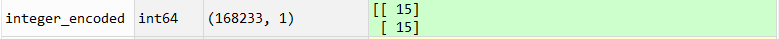
\includegraphics[width=8cm]{figures/1174084/7/7.png}
    \centering
    \caption{Hasil Praktek 7}
\end{figure}


\item Jelaskan kode program pada blok In[8]
\lstinputlisting[firstline=97, lastline=110]{src/1174084/7/1174084.py}
\begin{figure}[H]
    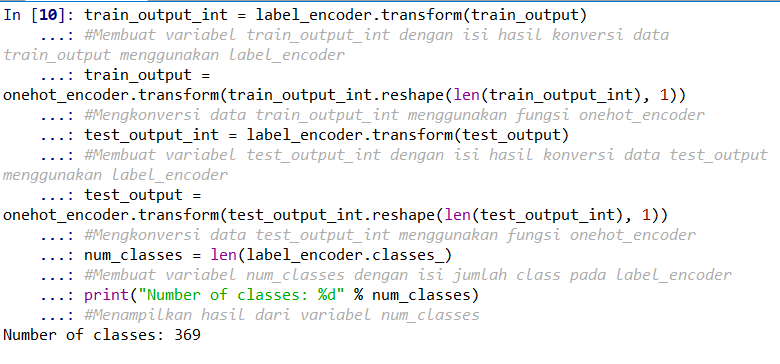
\includegraphics[width=8cm]{figures/1174084/7/8.png}
    \centering
    \caption{Hasil Praktek 8}
\end{figure}

\item Jelaskan kode program pada blok In[9]
\lstinputlisting[firstline=111, lastline=119]{src/1174084/7/1174084.py}
\begin{figure}[H]
    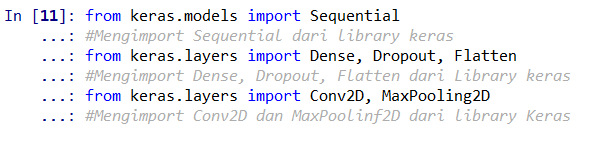
\includegraphics[width=12cm]{figures/1174084/7/9.png}
    \centering
    \caption{Hasil Praktek 9}
\end{figure}

\item Jelaskan kode program pada blok In[10]
\lstinputlisting[firstline=120, lastline=146]{src/1174084/7/1174084.py}	
\begin{figure}[H]
    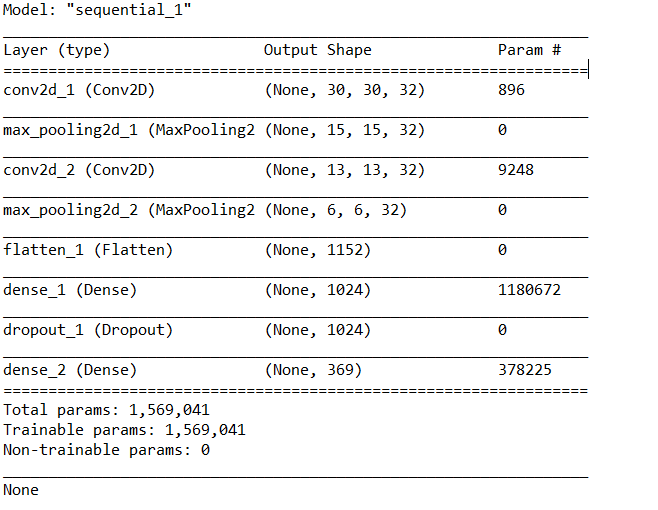
\includegraphics[width=8cm]{figures/1174084/7/10.png}
    \centering
    \caption{Hasil Praktek 10}
\end{figure}

\item Jelaskan kode program pada blok  In[11]
\lstinputlisting[firstline=147, lastline=153]{src/1174084/7/1174084.py}		
\begin{figure}[H]
    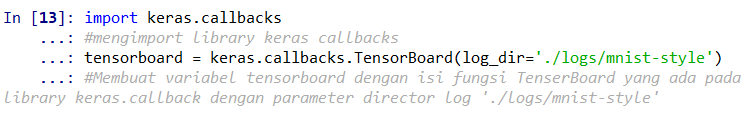
\includegraphics[width=8cm]{figures/1174084/7/11.png}
    \centering
    \caption{Hasil Praktek 11}
\end{figure}

\item Jelaskan kode program pada blok In[12]
\lstinputlisting[firstline=154, lastline=175]{src/1174084/7/1174084.py}	
\begin{figure}[H]
    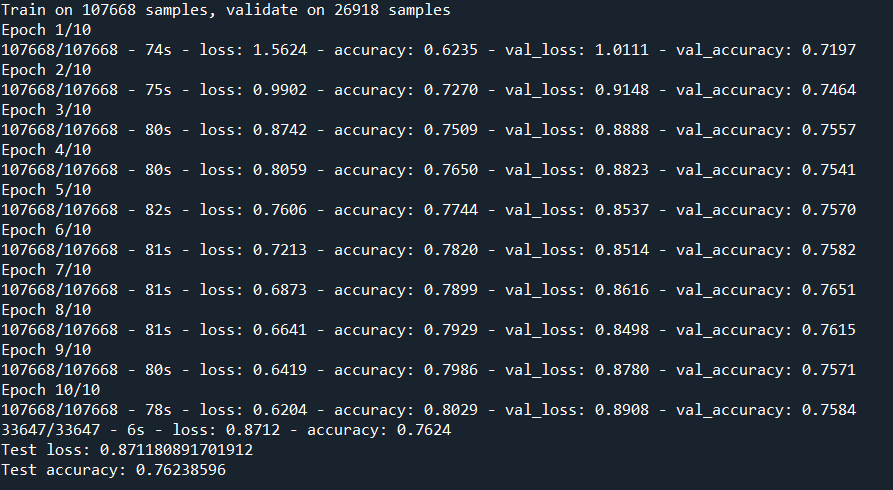
\includegraphics[width=8cm]{figures/1174084/7/12.png}
    \centering
    \caption{Hasil Praktek 12}
\end{figure}


\item Jelaskan kode program pada blok In[13]
\lstinputlisting[firstline=176, lastline=236]{src/1174084/7/1174084.py}	
\begin{figure}[H]
    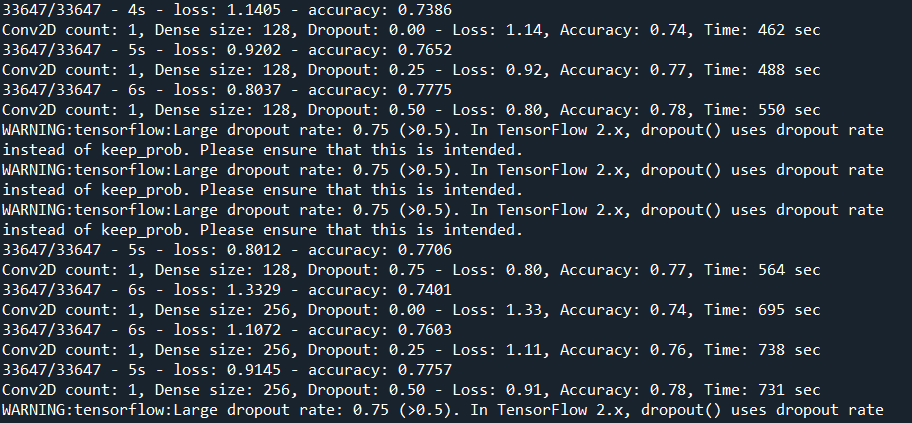
\includegraphics[width=8cm]{figures/1174084/7/13.png}
    \centering
    \caption{Hasil Praktek 13}
\end{figure}


\item Jelaskan kode program pada blok In[14]
\lstinputlisting[firstline=237, lastline=261]{src/1174084/7/1174084.py}	
\begin{figure}[H]
    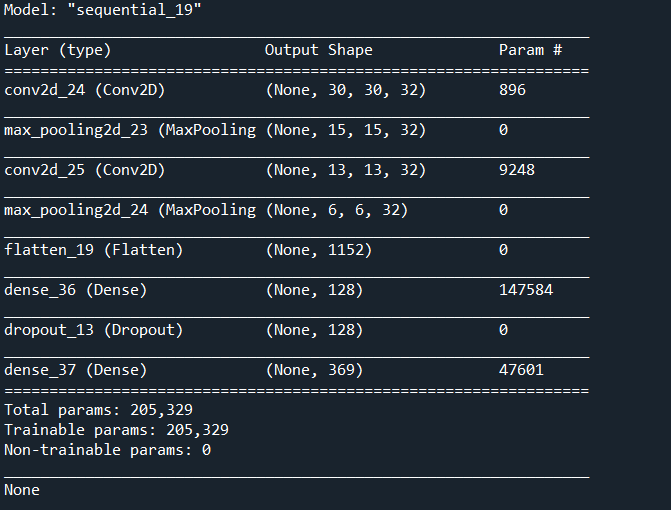
\includegraphics[width=8cm]{figures/1174084/7/14.png}
    \centering
    \caption{Hasil Praktek 14}
\end{figure}

\item Jelaskan kode program pada blok In[15]
\lstinputlisting[firstline=262, lastline=269]{src/1174084/7/1174084.py}	
\begin{figure}[H]
    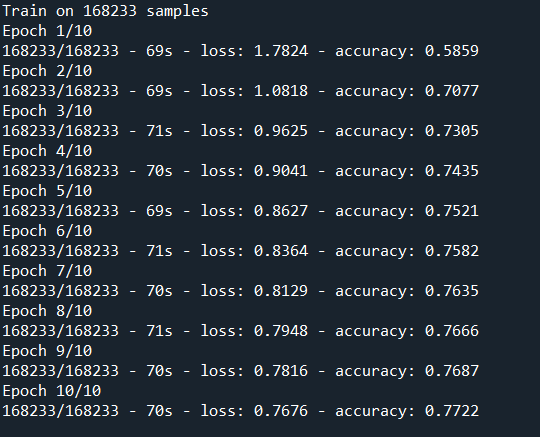
\includegraphics[width=8cm]{figures/1174084/7/15.png}
    \centering
    \caption{Hasil Praktek 15}
\end{figure}

\item Jelaskan kode program pada blok In[16]
\lstinputlisting[firstline=270, lastline=273]{src/1174084/7/1174084.py}	
\begin{figure}[H]
    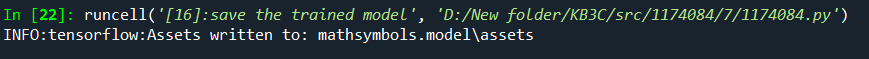
\includegraphics[width=8cm]{figures/1174084/7/16.png}
    \centering
    \caption{Hasil Praktek 16}
\end{figure}

\item Jelaskan kode program pada blok In[17]
\lstinputlisting[firstline=274, lastline=277]{src/1174084/7/1174084.py}	
\begin{figure}[H]
    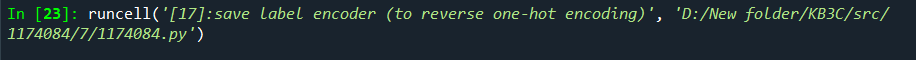
\includegraphics[width=8cm]{figures/1174084/7/17.png}
    \centering
    \caption{Hasil Praktek 17}
\end{figure}

\item Jelaskan kode program pada blok In[18]
\lstinputlisting[firstline=278, lastline=287]{src/1174084/7/1174084.py}	
\begin{figure}[H]
    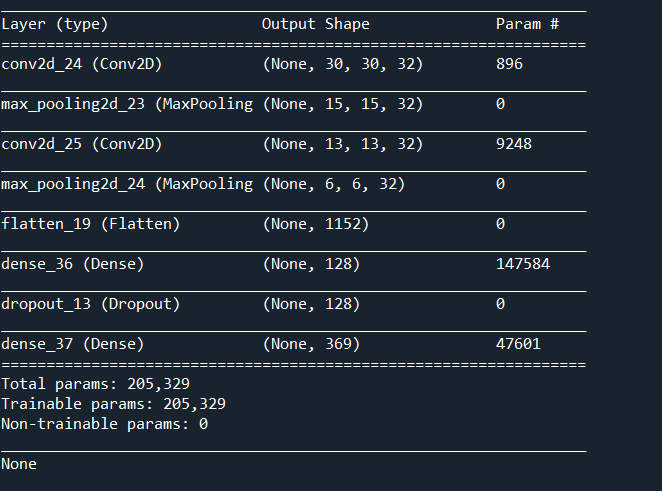
\includegraphics[width=8cm]{figures/1174084/7/18.png}
    \centering
    \caption{Hasil Praktek 18}
\end{figure}

\item Jelaskan kode program pada blok In[19]
\lstinputlisting[firstline=288, lastline=310]{src/1174084/7/1174084.py}	
\begin{figure}[H]
    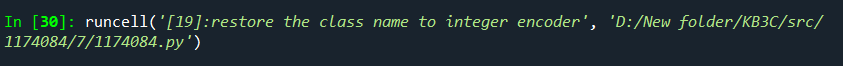
\includegraphics[width=8cm]{figures/1174084/7/19.png}
    \centering
    \caption{Hasil Praktek 19}
\end{figure}

\item Jelaskan kode program pada blok In[20]
\lstinputlisting[firstline=311, lastline=317]{src/1174084/7/1174084.py}	
\begin{figure}[H]
    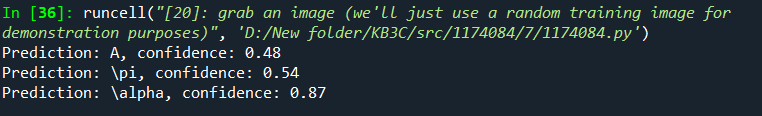
\includegraphics[width=8cm]{figures/1174084/7/20.png}
    \centering
    \caption{Hasil Praktek 20}
\end{figure}

\end{enumerate}


\subsection{Bukti Tidak Plagiat}
\begin{figure}[H]
	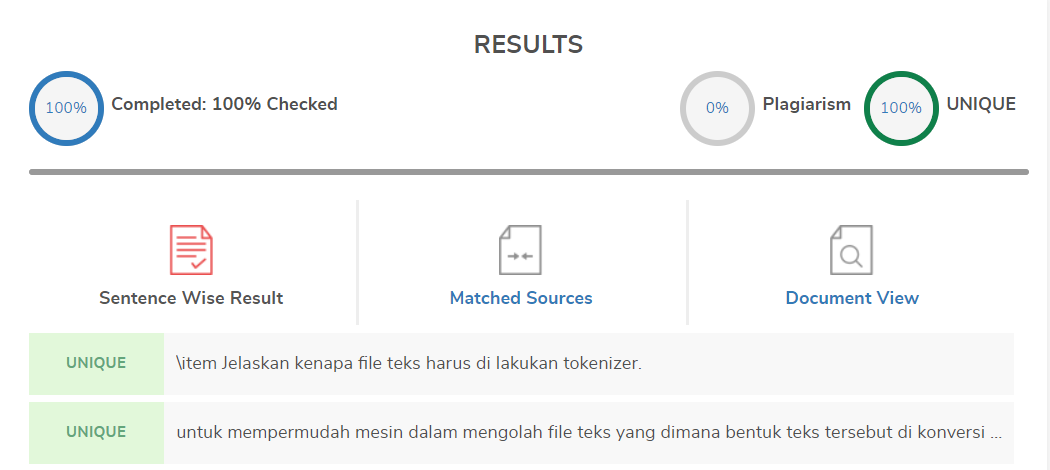
\includegraphics[width=4cm]{figures/1174084/7/plagiarism.png}
	\centering
	\caption{plagiarism}
\end{figure}


\subsection{Link Video Youtube}
https://youtu.be/djRkJBfOFJs

